
%(BEGIN_QUESTION)
% Copyright 2011, Tony R. Kuphaldt, released under the Creative Commons Attribution License (v 1.0)
% This means you may do almost anything with this work of mine, so long as you give me proper credit

This gas compressor is equipped with an override control system to ensure its suction line does not experience a vacuum, and that its drive motor does not become over-worked, as it attempts to maintain a constant discharge pressure:

$$\includegraphics[width=15.5cm]{i02509x01.eps}$$

Normally, control of the compressor's suction valve falls to the discharge pressure controller.  In the event that the motor power exceeds a pre-determined setpoint, or the suction controller detects a vacuum, either one of these constraint controllers will override the discharge pressure controller to maintain safe compressor operation at the expense of desired output pressure.

\filbreak

The control system for this compressor is a DCS, programmed using {\it function blocks}.  The function block diagram for this control scheme appears here, complete with ``live'' values showing the status of various signals at one point in time as the compressor is running:

$$\includegraphics[width=15.5cm]{i02509x02.eps}$$

Based on what you see here in this diagram, determine which controller is actually in control of the suction valve, and why.  Also, explain why all the ``back calculation'' signal lines are absolutely necessary for an override control system such as this to transition smoothly between override states (i.e. switch ``bumplessly'' from one selected controller to another).

\vskip 20pt \vbox{\hrule \hbox{\strut \vrule{} {\bf Suggestions for Socratic discussion} \vrule} \hrule}

\begin{itemize}
\item{} Can an instrument fault in this system shut the compressor off?  Why or why not?
\item{} Explain the purpose of the BKCAL signals in this system.
\item{} If this control strategy were implemented in FOUNDATION Fieldbus, where would you suggest locating the PID function blocks, and why?
\end{itemize}

\underbar{file i02509}
%(END_QUESTION)





%(BEGIN_ANSWER)

Back-calculation signal lines are essential for letting the non-selected function block(s) ``know'' what is going on ``downstream'' in the function block signal path.  Without these back-calculation lines in place, the de-selected control blocks would be completely unaware they were being de-selected, and would keep trying to control the process even though they had no control.

%(END_ANSWER)





%(BEGIN_NOTES)

Identities of each instrument in the block diagram, based on the selector blocks their respective PID blocks output to:

\begin{itemize}
\item{} {\bf PT-58} = Discharge pressure transmitter
\item{} {\bf PT-49} = Suction pressure transmitter
\item{} {\bf JT-51} = Motor power transmitter
\end{itemize}

The suction pressure controller is in control of the suction valve, overriding the discharge pressure controller.  We may tell this by the action of the high-select function block, which is selecting the output of the suction pressure controller (95\%) over the output of the discharge pressure controller (93\%).

\vskip 30pt

Note: this control strategy derived from diagram on page 130 of Francis G. Shinskey's {\it Energy Conservation Through Control}, copyright 1978.

%INDEX% Control, strategies: override control
%INDEX% DCS, programming: function block program
%INDEX% Process: compressor load control
%INDEX% Process troubleshooting: diagnosing problem via online function block display in DCS
%INDEX% Relay, computational: symbol identification

%(END_NOTES)


